\documentclass[letter]{article}
\usepackage{geometry}
\usepackage{graphicx}
\usepackage{natbib}
\usepackage{amsmath}
\usepackage{amssymb}
\usepackage{amsthm}
\usepackage{paralist}
\usepackage{epstopdf}
\usepackage{tabularx}
\usepackage{longtable}
\usepackage{multirow}
\usepackage{multicol}
\usepackage[hidelinks]{hyperref}
\usepackage{fancyvrb}
\usepackage{algorithm}
\usepackage{algorithmic}
\usepackage{float}
\usepackage{paralist}
\usepackage{tikz}
\usepackage[svgnames]{xcolor}
\usepackage{enumerate}
\usepackage{array}
\usepackage{times}
\usepackage{url}
\usepackage{fancyhdr}
\usepackage{comment}
\usepackage{environ}
\usepackage{times}
\usepackage{textcomp}
\usepackage{caption}

\usepackage{mathpazo}
\usepackage{domitian}
\usepackage[T1]{fontenc}
\let\oldstylenums\oldstyle

\urlstyle{rm}

\setlength\parindent{0pt} % Removes all indentation from paragraphs
\theoremstyle{definition}
\newtheorem{definition}{Definition}[]
\newtheorem{conjecture}{Conjecture}[]
\newtheorem{example}{Example}[]
\newtheorem{theorem}{Theorem}[]
\newtheorem{lemma}{Lemma}
\newtheorem{proposition}{Proposition}
\newtheorem{corollary}{Corollary}

\floatname{algorithm}{Procedure}
\renewcommand{\algorithmicrequire}{\textbf{Input:}}
\renewcommand{\algorithmicensure}{\textbf{Output:}}
\newcommand{\abs}[1]{\lvert#1\rvert}
\newcommand{\norm}[1]{\lVert#1\rVert}
\newcommand{\RR}{\mathbb{R}}
\newcommand{\CC}{\mathbb{C}}
\newcommand{\Nat}{\mathbb{N}}
\newcommand{\br}[1]{\{#1\}}
\DeclareMathOperator*{\argmin}{arg\,min}
\DeclareMathOperator*{\argmax}{arg\,max}
\renewcommand{\qedsymbol}{$\blacksquare$}

\definecolor{dkgreen}{rgb}{0,0.6,0}
\definecolor{gray}{rgb}{0.5,0.5,0.5}
\definecolor{mauve}{rgb}{0.58,0,0.82}

\newcommand{\Var}{\mathrm{Var}}
\newcommand{\Cov}{\mathrm{Cov}}

\newcommand{\vc}[1]{\boldsymbol{#1}}
\newcommand{\xv}{\vc{x}}
\newcommand{\Sigmav}{\vc{\Sigma}}
\newcommand{\alphav}{\vc{\alpha}}
\newcommand{\muv}{\vc{\mu}}

\newcommand{\red}[1]{\textcolor{red}{#1}}

\def\x{\mathbf x}
\def\y{\mathbf y}
\def\w{\mathbf w}
\def\v{\mathbf v}
\def\E{\mathbb E}
\def\V{\mathbb V}

% TO SHOW SOLUTIONS, include following (else comment out):
\newenvironment{soln}{
	\leavevmode\color{black}\ignorespaces
}{}


\hypersetup{
	%    colorlinks,
	linkcolor={red!50!black},
	citecolor={blue!50!black},
	urlcolor={blue!80!black}
}

\geometry{
	top=1in,            % <-- you want to adjust this
	inner=1in,
	outer=1in,
	bottom=1in,
	headheight=3em,       % <-- and this
	headsep=2em,          % <-- and this
	footskip=3em,
}


\pagestyle{fancyplain}
\lhead{\fancyplain{}{Homework 1}}
\rhead{\fancyplain{}{CS 760 Machine Learning}}
\cfoot{\thepage}

\title{\textsc{Homework 1}} % Title

%%% NOTE:  Replace 'NAME HERE' etc., and delete any "\red{}" wrappers (so it won't show up as red)

\author{
	  Gaurav Batra \\
	gbatra3@wisc.edu\\
} 

\date{}

\begin{document}
	
	\maketitle 
	
	
	\textbf{Instructions:} 
	This is a background self-test on the type of math we will encounter in class. If you find many questions intimidating, we suggest you drop 760 and take it again in the future when you are more prepared.
	
	You can use this latex file as a template to develop your homework.
	Submit your homework on time as a single pdf file to {\bf Gradescope}.
	There is no need to submit the latex source or any code.
	
	
	\section{Vectors and Matrices [6 pts]}
	Consider the matrix $X$ and the vectors $\mathbf{y}$ and $\textbf{z}$ below:
	$$
	X = \begin{pmatrix}
		3 & 2 \\ -7 & -5 \\
	\end{pmatrix}
	\qquad \mathbf{y} = \begin{pmatrix}
		2 \\ 1
	\end{pmatrix} \qquad \mathbf{z} = \begin{pmatrix}
		1 \\ -1
	\end{pmatrix}
	$$
	\begin{enumerate}
		\item 	Compute $\mathbf{y}^{T} X \mathbf{z}$\\
			
                \begin{soln}    
                    \textbf{Step 1: Compute $X \mathbf{z}$}\\
                    First, let's multiply the matrix $X$ with the vector $\mathbf{z}$:
                    \[
                    X \mathbf{z} = \begin{pmatrix} 3 & 2 \\ -7 & -5 \end{pmatrix} \begin{pmatrix} 1 \\ -1 \end{pmatrix}
                    = \begin{pmatrix} 3(1) + 2(-1) \\ -7(1) + (-5)(-1) \end{pmatrix}
                    = \begin{pmatrix} 3 - 2 \\ -7 + 5 \end{pmatrix}
                    = \begin{pmatrix} 1 \\ -2 \end{pmatrix}
                    \]
                    
                    \textbf{Step 2: Compute $\mathbf{y}^{T} (X \mathbf{z})$}\\
                    Next, we compute the dot product $\mathbf{y}^{T}$ and the result of $X \mathbf{z}$:
                    \[
                    \mathbf{y}^{T} = \begin{pmatrix} 2 & 1 \end{pmatrix}, \quad X \mathbf{z} = \begin{pmatrix} 1 \\ -2 \end{pmatrix}
                    \]
                    
                    Now, perform the dot product:
                    \[\mathbf{y}^{T} X \mathbf{z} = 2(1) + 1(-2) = 2 - 2 = 0\]
                    
                    Thus, the value of $\mathbf{y}^{T} X \mathbf{z}$ is 0.
                    
                \end{soln}

		\item 	Is $X$ invertible? If so, give the inverse, and if no, explain why not.\\
		

        \begin{soln}
        \textbf{A square matrix is invertible if and only if its determinant is non-zero.}
        
        Given the matrix $X$:
        \[
        X = \begin{pmatrix} 3 & 2 \\ -7 & -5 \end{pmatrix}
        \]
        
        The determinant of a $2 \times 2$ matrix $\begin{pmatrix} a & b \\ c & d \end{pmatrix}$ is given by:
        \[
        \det(X) = ad - bc
        \]
        
        In this case:
        \[
        \det(X) = (3)(-5) - (2)(-7) = -15 + 14 = -1
        \]
        
        Since the determinant of $X$ is $-1$, which is non-zero, $X$ is invertible.
        
        Now, the inverse of a $2 \times 2$ matrix $\begin{pmatrix} a & b \\ c & d \end{pmatrix}$ is given by:
        \[
        X^{-1} = \frac{1}{\det(X)} \begin{pmatrix} d & -b \\ -c & a \end{pmatrix}
        \]
        
        Substitute the values for $a = 3$, $b = 2$, $c = -7$, and $d = -5$:
        \[
        X^{-1} = \frac{1}{-1} \begin{pmatrix} -5 & -2 \\ 7 & 3 \end{pmatrix} = \begin{pmatrix} 5 & 2 \\ -7 & -3 \end{pmatrix}
        \]
        
        Thus, the inverse of $X$ is:
        \[
        X^{-1} = \begin{pmatrix} 5 & 2 \\ -7 & -3 \end{pmatrix}
        \]
        \end{soln}

	\end{enumerate}

 \pagebreak
	
	\section{Calculus [3 pts]}
	\begin{enumerate}
		\item If $y = e^{-x} + \arctan(z)x^{6/z} - \ln\cfrac{x}{x+1}$, what is the partial derivative of $y$ with respect to $x$?\\
		\begin{soln}
        
        
        Given:
        \[
        y = e^{-x} + \arctan(z)x^{6/z} - \ln\left(\frac{x}{x+1}\right)
        \]
        
        We will differentiate each term with respect to $x$, treating $z$ as a constant.
        
        \textbf{Term 1:} $e^{-x}$\\
        The derivative of $e^{-x}$ is:
        \[
        \frac{\partial}{\partial x} \left( e^{-x} \right) = -e^{-x}
        \]
        
        \textbf{Term 2:} $\arctan(z)x^{6/z}$\\
        Using the power rule:
        \[
        \frac{\partial}{\partial x} \left( x^{6/z} \right) = \frac{6}{z} x^{(6/z) - 1}
        \]
        Thus, the derivative of the second term is:
        \[
        \frac{\partial}{\partial x} \left( \arctan(z) x^{6/z} \right) = \arctan(z) \cdot \frac{6}{z} x^{(6/z) - 1}
        \]
        
        \textbf{Term 3:} $-\ln\left(\frac{x}{x+1}\right)$\\
        Simplify:
        \[
        \ln\left(\frac{x}{x+1}\right) = \ln(x) - \ln(x+1)
        \]
        Thus, the derivative is:
        \[
        \frac{\partial}{\partial x} \left( - \ln\left(\frac{x}{x+1}\right) \right) = -\left( \frac{1}{x} - \frac{1}{x+1} \right)
        \]
        
        \textbf{Final Result:}\\
        Summing the derivatives:
        \[
        \frac{\partial y}{\partial x} = -e^{-x} + \arctan(z) \cdot \frac{6}{z} x^{(6/z) - 1} - \left( \frac{1}{x} - \frac{1}{x+1} \right)
        \]
        \end{soln}
	\end{enumerate}
	
	
\pagebreak	
	
	\section{Probability and Statistics [10 pts]}
	Consider a sequence of data $S = (1, 1, 1, 0, 1)$ created by flipping a coin $x$ five times, where 0 denotes that the coin turned up heads and 1 denotes that it turned up tails.
	\begin{enumerate}
		\item 	(2.5 pts) What is the probability of observing this data, assuming it was generated by flipping a biased coin with $p(x=1) = 0.6$?
		
		\begin{soln}
            The probability of flipping heads is $p(x=0) = 1 - 0.6 = 0.4$. The probability of observing the entire sequence is the product of the probabilities of each individual outcome, assuming independent flips.
            
            
            \[
            P(S) = p(x_1=1) \cdot p(x_2=1) \cdot p(x_3=1) \cdot p(x_4=0) \cdot p(x_5=1)
            \]
            Substituting the probabilities:
            \[
            P(S) = (0.6) \cdot (0.6) \cdot (0.6) \cdot (0.4) \cdot (0.6)
            \]
            \[
            P(S) = (0.6)^4 \cdot (0.4) = 0.1296 \cdot 0.4 = 0.05184
            \]
            
            Thus, the probability of observing the sequence $S$ is:
            \[
            P(S) = 0.05184
            \]
            \end{soln}
		
    		\item 	(2.5 pts) Note that the probability of this data sample could be greater if the value of $p(x = 1)$ was not $0.6$, but instead some other value. What is the value that maximizes the probability of $S$? Please justify your answer.\\

		\begin{soln}
            The sequence $S$ contains 4 tails (denoted by 1) and 1 head (denoted by 0). The probability of observing this sequence is:
            \[
            P(S) = p^4 (1 - p)
            \]
            where $p^4$ represents the probability of getting 4 tails, and $(1 - p)$ represents the probability of getting 1 head.
            
            To maximize $P(S)$, we take the derivative of $P(S)$ with respect to $p$ and set it equal to 0. Let:
            \[
            P(p) = p^4 (1 - p)
            \]
            Differentiate $P(p)$ using the product rule:
            \[
            \frac{dP(p)}{dp} = \frac{d}{dp} \left( p^4 \cdot (1 - p) \right) = \frac{d}{dp} \left( p^4 \right) \cdot (1 - p) + p^4 \cdot \frac{d}{dp} (1 - p)
            \]
            This simplifies to:
            \[
            \frac{dP(p)}{dp} = 4p^3 (1 - p) - p^4
            \]
            
            Set the derivative equal to 0:
            \[
            4p^3 (1 - p) - p^4 = 0
            \]
            Factor the equation:
            \[
            p^3 (4 - 5p) = 0
            \]
            This gives two solutions: $p = 0$ and $p = \frac{4}{5}$. Since $p = 0$ is not realistic in this context, the value that maximizes the probability is:
            \[
            p = \frac{4}{5}
            \]
            
            Thus, the value of $p$ that maximizes the probability of observing the sequence $S$ is $p = \frac{4}{5}$.
            \end{soln}
		
		\item 	(5 pts) Consider the following joint probability table where both $A$ and $B$ are binary random variables: 
		\begin{table}[htb]
			\centering
			\begin{tabular}{ccc}\hline
				A & B & $P(A, B)$  \\\hline
				0 & 0 & 0.3 \\
				0 & 1 & 0.1 \\
				1 & 0 & 0.1 \\
				1 & 1 & 0.5 \\\hline
			\end{tabular}
		\end{table}
		\begin{enumerate}
			\item 	What is $P(A = 0 | B = 1)$?\\
			\begin{soln}
                \[
                P(A = 0 \mid B = 1) = \frac{P(A = 0, B = 1)}{P(B = 1)}
                \]
                From the table:
                \[
                P(A = 0, B = 1) = 0.1
                \]
                Next, we compute $P(B = 1)$:
                \[
                P(B = 1) = P(A = 0, B = 1) + P(A = 1, B = 1) = 0.1 + 0.5 = 0.6
                \]
                Thus, the conditional probability is:
                \[
                P(A = 0 \mid B = 1) = \frac{0.1}{0.6} = \frac{1}{6}
                \]
                \end{soln}
			 
			\item 	What is $P(A = 1 \vee B = 1 )$?\\
		      \begin{soln}
                \[
                P(A = 1 \vee B = 1) = P(A = 1) + P(B = 1) - P(A = 1, B = 1)
                \]
                From the table:
                \[
                P(A = 1) = P(A = 1, B = 0) + P(A = 1, B = 1) = 0.1 + 0.5 = 0.6
                \]
                We already know that $P(B = 1) = 0.6$, and from the table:
                \[
                P(A = 1, B = 1) = 0.5
                \]
                Thus:
                \[
                P(A = 1 \vee B = 1) = 0.6 + 0.6 - 0.5 = 0.7
                \]
                \end{soln}
		\end{enumerate}
	\end{enumerate}

\pagebreak
	\section{Big-O Notation [6 pts]}
	For each pair $(f, g)$ of functions below, list which of the following
	are true: $f(n) = O(g(n))$, $g(n) = O(f(n))$, both, or
	neither. Briefly justify your answers.
	\begin{enumerate}
		\item 	$f(n) = \ln(n)$, $g(n) = \log_{2}(n)$.\\
    		\begin{soln}
                \[
                \log_2(n) = \frac{\ln(n)}{\ln(2)}
                \]
                Thus, $\ln(n)$ and $\log_2(n)$ differ by a constant factor $\ln(2)$, which does not affect asymptotic growth.
                
                $f(n) = \ln(n) = O(\log_2(n))$\\
                
                Since $\ln(n)$ is a constant multiple of $\log_2(n)$, we have $f(n) = O(g(n))$.
                
                $g(n) = \log_2(n) = O(\ln(n))$\\
                
                Similarly, $\log_2(n)$ is a constant multiple of $\ln(n)$, so $g(n) = O(f(n))$.
                
                
                Therefore, both $f(n) = O(g(n))$ and $g(n) = O(f(n))$ are true.
                \end{soln}

                \begin{figure}[H]
                    \centering
                    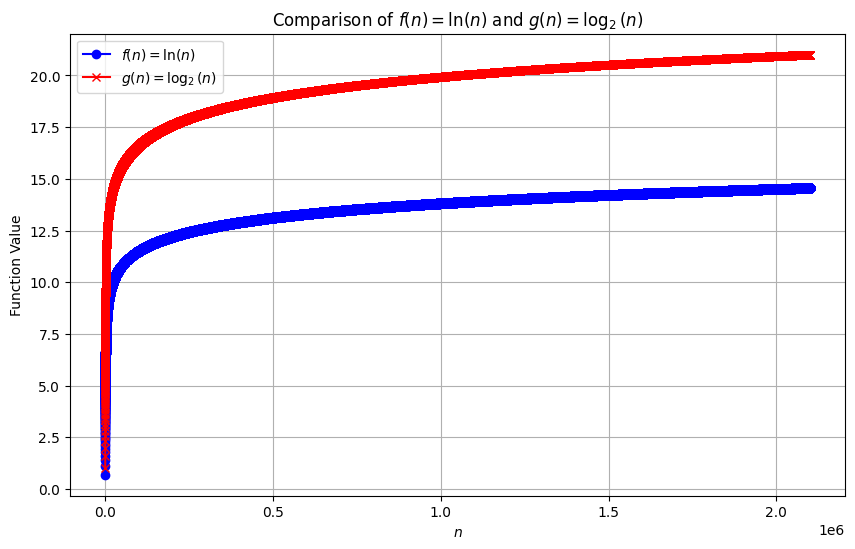
\includegraphics[width=0.8\textwidth]{big-o-1.png} % Replace with the path to your image
                    \caption{Comparison of $f(n) = \ln(n)$ and $g(n) = \log_{2}(n)$. The plot shows that $f(n)$ and $g(n)$ grow at the same rate up to a constant factor.}
                    \label{fig:ln_vs_log2}
                \end{figure}

                

    		
		\item 	$f(n) =  \log_{2}\log_{2}(n)$, $g(n) = \log_{2}(n)$.\\
		\begin{soln}
            
            \textbf{1. Is $f(n) = O(g(n))$?}\\
            To show $f(n) = O(g(n))$, we need to verify if:
            \[
            \log_{2} \log_{2}(n) \leq C \cdot \log_{2}(n)
            \]
            for some constant $C$ and sufficiently large $n$. Since $\log_{2} \log_{2}(n)$ grows much slower than $\log_{2}(n)$, this inequality will hold true. Thus:
            \[
            \log_{2} \log_{2}(n) = O(\log_{2}(n))
            \]
            
            \textbf{2. Is $g(n) = O(f(n))$?}\\
            To show $g(n) = O(f(n))$, we need to check if:
            \[
            \log_{2}(n) \leq C \cdot \log_{2} \log_{2}(n)
            \]
            for some constant $C$ and sufficiently large $n$. Since $\log_{2}(n)$ grows faster than $\log_{2} \log_{2}(n)$, there does not exist such a constant $C$ that satisfies this inequality. Thus:
            \[
            \log_{2}(n) \neq O(\log_{2} \log_{2}(n))
            \]
            
            Therefore, $f(n) = O(g(n))$ but $g(n) \neq O(f(n))$.
            \end{soln}

            \begin{figure}[H]
                \centering
                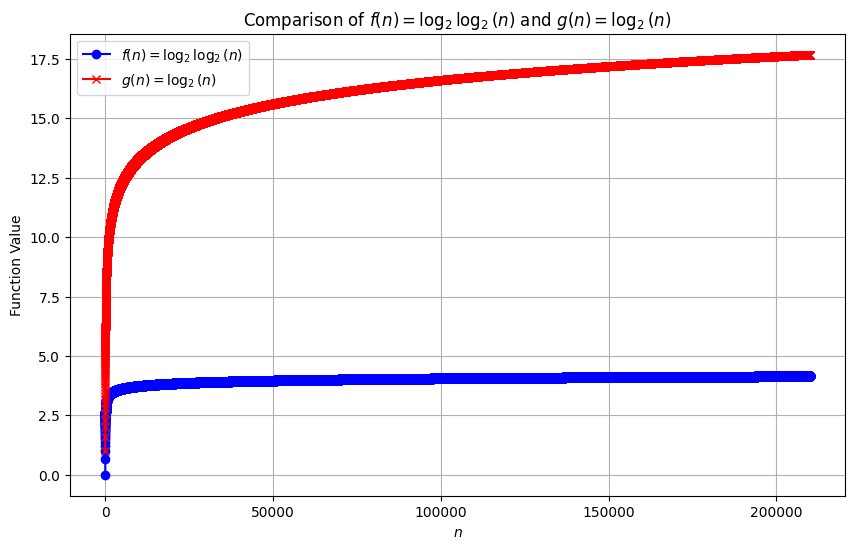
\includegraphics[width=0.8\textwidth]{big-o-2.png} % Replace with the path to your image
                \caption{Comparison of $f(n) = \log_{2} \log_{2}(n)$ and $g(n) = \log_{2}(n)$. The plot shows that $f(n)$ grows much slower than $g(n)$.}
                \label{fig:log2_log2_vs_log2}
            \end{figure}

		
		\item 	$f(n) = n!$, $g(n) = 2^n$.\\
		\begin{soln}
            
            \textbf{1. Is $f(n) = O(g(n))$?}\\
            To determine if $f(n) = O(g(n))$, we need to check if there exists a constant $C$                                   such that:
            \[
            n! \leq C \cdot 2^n
            \]
            Using Stirling's approximation:
            \[
            n! \approx \sqrt{2 \pi n} \left(\frac{n}{e}\right)^n
            \]
            We compare:
            \[
            \frac{n!}{2^n} \approx \sqrt{2 \pi n} \left(\frac{n}{2e}\right)^n
            \]
            For large $n$, $\left(\frac{n}{2e}\right)^n$ grows without bound, so $n!$ grows faster than $2^n$. Hence, $n! \neq O(2^n)$.
            
            \textbf{2. Is $g(n) = O(f(n))$?}\\
            To determine if $g(n) = O(f(n))$, we need to check if:
            \[
            2^n \leq C \cdot n!
            \]
            Since $n!$ grows faster than $2^n$, there will always be some constant $C$ such that this inequality holds for sufficiently large $n$. Thus:
            \[
            2^n = O(n!)
            \]
            
            Therefore, $f(n) = n!$ is not $O(g(n))$, but $g(n) = 2^n$ is $O(f(n))$.
            \end{soln}


            \begin{figure}[H]
                \centering
                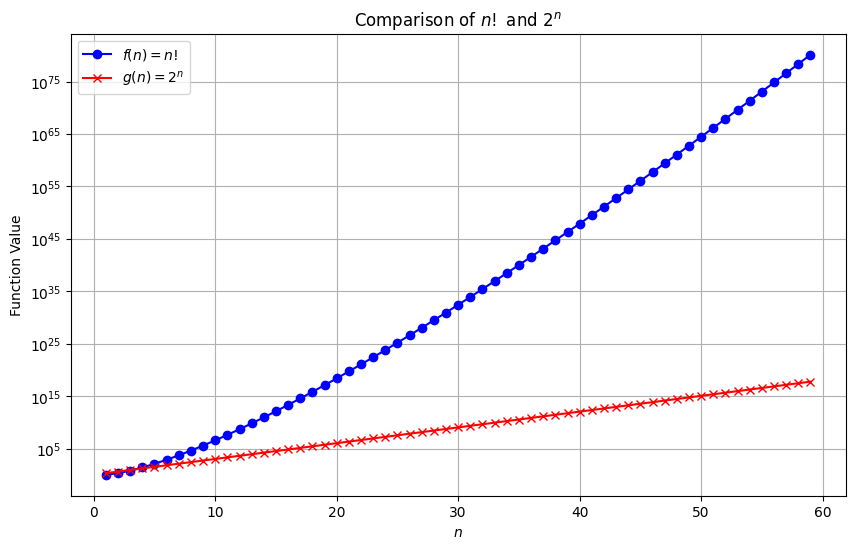
\includegraphics[width=0.8\textwidth]{big-o-3.png} % Replace with the path to your image
                \caption{Comparison of $n!$ and $2^n$. The plot shows that $n!$ grows much faster than $2^n$ for larger values of $n$.}
                \label{fig:factorial_vs_exponential}
            \end{figure}

	\end{enumerate}
	
	
	
\pagebreak	
	
	\section{Probability and Random Variables }
	\subsection{Probability [12.5 pts]}
	State true or false. Here $\Omega$ denotes the sample space and $A^c$ denotes the complement of the event $A$.
	\begin{enumerate}
		\item For any $A, B \subseteq \Omega$, $P(A|B)P(A) = P(B|A)P(B)$.\\
		
            \begin{soln}
                The statement is \textbf{false}.
                
                \textbf{Explanation:} The correct form of this relation is Bayes' Theorem, which states:
                \[
                P(A|B)P(B) = P(B|A)P(A)
                \]
                This equation indicates that \( P(A|B) \) is the conditional probability of \( A \) given \( B \), and it is equal to the conditional probability of \( B \) given \( A \), scaled by their respective unconditional probabilities \( P(A) \) and \( P(B) \).
            \end{soln}
		
		\item For any $A, B \subseteq \Omega$, $P(A \cup B) = P(A) + P(B) - P(B \cap A)$.\\         
		
            \begin{soln}
                The statement is \textbf{true}.
                
                \textbf{Explanation:} This is the formula for the probability of the union of two events, which accounts for the overlap between the events. The inclusion-exclusion principle is applied here to avoid double-counting the probability of the intersection \( P(A \cap B) \), which appears in both \( P(A) \) and \( P(B) \). Therefore, the correct expression for the probability of \( A \cup B \) is:
                \[
                P(A \cup B) = P(A) + P(B) - P(A \cap B)
                \]
            \end{soln}
		
		\item For any $A, B, C \subseteq \Omega$ such that $P(B \cup C) > 0$,
		$\frac{P(A \cup B \cup C)}{P(B \cup C)} \geq P(A | B \cup C) P(B)$.\\ 
		
            \begin{soln}
            The statement is \textbf{true}.

            % We can rewrite the right-hand side of the inequality as follows:
            % \[
            % P(A | B \cup C) P(B) = \frac{P(A \cap (B \cup C))}{P(B \cup C)} \cdot P(B)
            % \]
        
            % left-hand side of the inequality:
            % \[
            % \frac{P(A \cup B \cup C)}{P(B \cup C)}
            % \]
        
            % As,
            % \[
            % P(A \cup B \cup C) = P(A) + P(B \cup C) - P(A \cap (B \cup C))
            % \]
        
            % Therefore:
            % \[
            % \frac{P(A \cup B \cup C)}{P(B \cup C)} = \frac{P(A) + P(B \cup C) - P(A \cap (B \cup C))}{P(B \cup C)}
            % \]
        
            % Now we need to show:
            % \[
            % \frac{P(A \cup B \cup C)}{P(B \cup C)} \geq P(A | B \cup C) P(B)
            % \]
        
            % Substituting the simplified expressions:
            % \[
            % \frac{P(A) + P(B \cup C) + P(A \cap (B \cup C))}{P(B \cup C)} \geq P(A \cap (B \cup C)) \cdot \frac{P(B)}{P(B \cup C)}
            % \]
        
            % Therefore:
            % \[
            % P(A) + P(B \cup C) \geq (P(B) - 1)\cdot[P(A \cap (B \cup C))]
            % \]
        
            % Given that \( P(B) \leq 1 \), \( P(A \cap (B \cup C)) \geq 0\) and \( P(A) + P(B \cup C) \geq 0\), the inequality holds true. 
        
            % Therefore, the inequality is valid:
            % \[
            % \frac{P(A \cup B \cup C)}{P(B \cup C)} \geq P(A | B \cup C) P(B)
            % \]
        
            
            \end{soln}

		
		\item For any $A, B\subseteq\Omega$ such that $P(B) > 0, P(A^c) > 0$,
		$P(B|A^C) + P(B|A) = 1$.\\ 
		
            
            \begin{soln}
            This statement is \textbf{false}.

            \textbf{Counterexample:}
            
            Consider the following probabilities:
            \begin{itemize}
                \item $P(B) = 0.8$
                \item $P(A) = 0.3$
                \item $P(A \cap B) = 0.2$
            \end{itemize}
            
            We will calculate whether $P(B | A^c) + P(B | A) = 1$ holds:
            
            \begin{enumerate}
                \item Calculate $P(B | A)$:
                \[
                P(B | A) = \frac{P(B \cap A)}{P(A)} = \frac{0.2}{0.3} = \frac{2}{3} \approx 0.6667
                \]
            
                \item Calculate $P(A^c)$:
                \[
                P(A^c) = 1 - P(A) = 1 - 0.3 = 0.7
                \]
            
                \item Find $P(B \cap A^c)$:
                \[
                P(B \cap A^c) = P(B) - P(B \cap A) = 0.8 - 0.2 = 0.6
                \]
            
                \item Calculate $P(B | A^c)$:
                \[
                P(B | A^c) = \frac{P(B \cap A^c)}{P(A^c)} = \frac{0.6}{0.7} \approx 0.8571
                \]
            
                \item Check if $P(B | A^c) + P(B | A) = 1$:
                \[
                P(B | A) + P(B | A^c) \approx 0.6667 + 0.8571 = 1.5238
                \]
            
                Since $1.5238 \neq 1$, the statement $P(B | A^c) + P(B | A) = 1$ does not hold. Therefore, the statement is \textbf{false}.
            \end{enumerate}
            \end{soln}
		
		\item If $A$ and $B$ are independent events, then $A^{c}$ and $B^{c}$ are independent.\\
		\begin{soln}
            
            This statement is \textbf{true}.
            
            \textbf{Proof:}
            
            Start with the independence of $A$ and $B$. By definition, if $A$ and $B$ are independent, then:
            \[
            P(A \cap B) = P(A) \cdot P(B)
            \]
            
            Using De Morgan's law:
            \[
            A^c \cap B^c = (A \cup B)^c
            \]
            Thus:
            \[
            P(A^c \cap B^c) = 1 - P(A \cup B)
            \]

            Calculate $P(A^c)$ and $P(B^c)$:
            \[
            P(A^c) = 1 - P(A)
            \]
            \[
            P(B^c) = 1 - P(B)
            \]

            Compute $P(A^c) \cdot P(B^c)$:
            \[
            P(A^c) \cdot P(B^c) = (1 - P(A)) \cdot (1 - P(B))
            \]
            \[
            P(A^c) \cdot P(B^c) = 1 - P(A) - P(B) + P(A) \cdot P(B)
            \]
            \[
            P(A^c) \cdot P(B^c) = 1 - P(A \cup B) = P(A^c \cap B^c)
            \]
            Thus, $P(A^c \cap B^c) = P(A^c) \cdot P(B^c)$, proving that $A^c$ and $B^c$ are independent.
            \end{soln}
		
	\end{enumerate}
	
	\subsection{Discrete and Continuous Distributions [12.5 pts]}
	Match the distribution name to its probability density / mass
	function.
	\begin{enumerate}[(a)]
		\begin{minipage}{0.4\linewidth}
			\item Gamma \begin{soln} : j \end{soln}
			\item Multinomial  \begin{soln} : i \end{soln}
			\item Laplace \begin{soln}  : h \end{soln}
			\item Poisson \begin{soln}  : l \end{soln}
			\item Dirichlet  \begin{soln}  : k \end{soln}
		\end{minipage}
  \quad
		\begin{minipage}{0.5\linewidth}
			\item $f(\xv; \Sigmav, \muv) = \frac{1}{\sqrt{(2\pi)^k \mathrm{det}(\Sigmav) }} \exp\left( -\frac{1}{2}
			(\xv - \muv)^T \Sigmav^{-1} (\xv - \muv)  \right)$
			\item $f(x; n, \alpha) = \binom{n}{x} \alpha^x (1 - \alpha)^{n-x}$
			for $x \in \{0,\ldots, n\}$; $0$ otherwise
			\item $f(x; b, \mu) = \frac{1}{2b} \exp\left( - \frac{|x - \mu|}{b} \right)$
			\item $f(\xv; n, \alphav) = \frac{n!}{\Pi_{i=1}^k x_i!}
			\Pi_{i=1}^k \alpha_i^{x_i}$ for $x_i \in \{0,\ldots,n\}$ and
			$\sum_{i=1}^k x_i = n$; $0$ otherwise
			\item $f(x; \alpha, \beta) = \frac{\beta^{\alpha}}{\Gamma(\alpha)} x^{\alpha -
				1}e^{-\beta x}$ for $x \in (0,+\infty)$; $0$ otherwise
			\item $f(\xv; \alphav) = \frac{\Gamma(\sum_{i=1}^k
				\alpha_i)}{\prod_{i=1}^k \Gamma(\alpha_i)} \prod_{i=1}^{k}
			x_i^{\alpha_i - 1}$ for $x_i \in (0,1)$ and $\sum_{i=1}^k x_i =
			1$; 0 otherwise
			\item $f(x; \lambda) = \lambda^x \frac{e^{-\lambda}}{x!}$ for all
			$x \in Z^+$; $0$ otherwise
		\end{minipage}
	\end{enumerate}
	
	\subsection{Mean and Variance [10 pts]}
	\begin{enumerate}
		\item Consider a random variable which follows a Binomial
		distribution: $X \sim \text{Binomial}(n, p)$.
		\begin{enumerate}
			\item What is the mean of the random variable?\\
			
                \begin{soln}
				\[
				E[X] = \sum_{k=0}^{n} k \cdot P(X = k)
				\]
				
				For a Binomial random variable, the probability mass function is:
				\[
				P(X = k) = \binom{n}{k} p^k (1 - p)^{n - k}
				\]
				
				Substituting this into the expectation formula, we get:
				\[
				E[X] = \sum_{k=0}^{n} k \cdot \binom{n}{k} p^k (1 - p)^{n - k}
				\]
				
				Using the identity \( k \cdot \binom{n}{k} = n \cdot \binom{n - 1}{k - 1} \), we rewrite the sum as:
				\[
				E[X] = \sum_{k=0}^{n} n \cdot \binom{n - 1}{k - 1} p^k (1 - p)^{n - k}
				\]
				
				Factoring out \( n \):
				\[
				E[X] = n \sum_{k=1}^{n} \binom{n - 1}{k - 1} p^k (1 - p)^{n - k}
				\]
				
				Changing the index of summation from \( k \) to \( j = k - 1 \), we get:
				\[
				E[X] = n p \sum_{j=0}^{n - 1} \binom{n - 1}{j} p^j (1 - p)^{n - 1 - j}
				\]
				
				This is the binomial expansion of \( (p + (1 - p))^{n - 1} \):
				\[
				E[X] = n p \cdot 1 = np
				\]
				
				Thus, the mean of \( X \) is:
				\[
				E[X] = np
				\]
			\end{soln}
			\item What is the variance of the random variable?\\
			
                \begin{soln}
                The variance of $X$ is given by:
                \[
                \Var(X) = E[X^2] - (E[X])^2
                \]
                
                We know the following:
                \[
                E[X] = np
                \]
                
                Also:
                \[
                E[X^2] = E[X(X - 1)] + E[X]
                \]
                  
                To find the expectation $E[X(X - 1)]$, where $X \sim \text{Binomial}(n, p)$. The binomial random variable $X$ counts the number of successes in $n$ independent Bernoulli trials, each with success probability $p$. Using indicator variables, we can express $X$ as:
                \[
                X = I_1 + I_2 + \dots + I_n
                \]
                where $I_i = 1$ if trial $i$ is a success, and $I_i = 0$ otherwise.
                
                Thus, $X(X - 1)$ can be expanded as:
                \[
                X(X - 1) = \sum_{i=1}^{n} \sum_{j \neq i} I_i I_j
                \]
                
                The expectation $E[I_i I_j]$ for independent trials $i$ and $j$ is:
                \[
                E[I_i I_j] = p^2
                \]
                since $P(\text{both trials are successes}) = p^2$.
                
                There are $n(n-1)$ pairs of distinct trials, so:
                \[
                E[X(X-1)] = n(n-1) p^2
                \]
                
                Now, using this in the expression for $E[X^2]$:
                \[
                E[X^2] = E[X(X - 1)] + E[X] = n(n-1)p^2 + np = n^2p^2 + np(1-p)
                \]
                
                Finally, substituting into the formula for variance:
                \[
                \Var(X) = E[X^2] - (E[X])^2 = n^2p^2 + np(1 - p) - (np)^2 = np(1 - p)
                \]
                
                Thus, the variance of $X$ is:
                \[
                \Var(X) = np(1 - p)
                \]
                \end{soln}
		\end{enumerate}
		
		\item Let $X$ be a random variable and
		$\mathbb{E}[X] = 1, \Var(X) = 1$. Compute the following values:
		\begin{enumerate}
			\item $\mathbb{E}[5X]$\\
			
                \begin{soln}
			\[
			\mathbb{E}[aX] = a \cdot \mathbb{E}[X]
			\]
			
			Here, $a = 5$, so:
			\[
			\mathbb{E}[5X] = 5 \cdot \mathbb{E}[X]
			\]
			\[
			\mathbb{E}[5X] = 5 \cdot 1 = 5
			\]
		      \end{soln}
			\item $\Var(5X)$\\
			\begin{soln}
			\[
			\Var(aX) = a^2 \cdot \Var(X)
			\]
			
			Here, $a = 5$, so:
			\[
			\Var(5X) = 5^2 \cdot \Var(X)
			\]
			\[
			\Var(5X) = 25 \cdot 1 = 25
			\]
		      \end{soln}
			\item $\Var(X+5)$\\
			\begin{soln}
			\[
			\Var(X + c) = \Var(X)
			\]
			
		 Here, $c = 5$, so:
			\[
			\Var(X + 5) = \Var(X) = 1
			\]
		      \end{soln}
		\end{enumerate}
	\end{enumerate}
	
	%\clearpage
	
	\subsection{Mutual and Conditional Independence [12 pts]}
	\begin{enumerate}
		\item (3 pts) If $X$ and $Y$ are independent random variables, show that
		$\mathbb{E}[XY] = \mathbb{E}[X]\mathbb{E}[Y]$.
		
		\begin{soln}
			\[
			\mathbb{E}[XY] = \int_{-\infty}^{\infty} \int_{-\infty}^{\infty} xy \, f_{X,Y}(x, y) \, dx \, dy
			\]
			
			where \(f_{X,Y}(x, y)\) is the joint probability density function of \(X\) and \(Y\). 
			
			For independent random variables \(X\) and \(Y\), the joint probability density function factors into the product of the marginal density functions:
			
			\[
			f_{X,Y}(x, y) = f_X(x) f_Y(y)
			\]
			
			Substituting this into the expectation formula:
			
			\[
			\mathbb{E}[XY] = \int_{-\infty}^{\infty} \int_{-\infty}^{\infty} xy \, f_X(x) f_Y(y) \, dx \, dy
			\]
			
			We can separate the integrals since \(f_X(x)\) and \(f_Y(y)\) are functions of \(x\) and \(y\) respectively:
			
			\[
			\mathbb{E}[XY] = \left( \int_{-\infty}^{\infty} x f_X(x) \, dx \right) \left( \int_{-\infty}^{\infty} y f_Y(y) \, dy \right)
			\]
			
			The first integral is the definition of the expectation of \(X\):
			
			\[
			\mathbb{E}[X] = \int_{-\infty}^{\infty} x f_X(x) \, dx
			\]
			
			The second integral is the definition of the expectation of \(Y\):
			
			\[
			\mathbb{E}[Y] = \int_{-\infty}^{\infty} y f_Y(y) \, dy
			\]
			
			Thus:
			
			\[
			\mathbb{E}[XY] = \mathbb{E}[X] \cdot \mathbb{E}[Y]
			\]
		\end{soln}
		
		\item (3 pts) If $X$ and $Y$ are independent random variables, show that
		$\Var(X+Y) = \Var(X) + \Var(Y)$. \\
		Hint: $\Var(X+Y) = \Var(X) + 2\Cov(X, Y) + \Var(Y)$
		
		\begin{soln}
			\[
			\Var(X + Y) = \mathbb{E}[(X + Y)^2] - (\mathbb{E}[X + Y])^2
			\]
			
			
			
			\[
			(X + Y)^2 = X^2 + 2XY + Y^2
			\]
			
			Thus:
			
			\[
			\mathbb{E}[(X + Y)^2] = \mathbb{E}[X^2 + 2XY + Y^2]
			\]
			
			Using the linearity of expectation:
			
			\[
			\mathbb{E}[X^2 + 2XY + Y^2] = \mathbb{E}[X^2] + \mathbb{E}[2XY] + \mathbb{E}[Y^2]
			\]
			
			\[
			\mathbb{E}[X^2 + 2XY + Y^2] = \mathbb{E}[X^2] + 2 \mathbb{E}[XY] + \mathbb{E}[Y^2]
			\]
			
			To compute \(\mathbb{E}[XY]\) for independent random variables \(X\) and \(Y\):
			
			\[
			\mathbb{E}[XY] = \mathbb{E}[X] \cdot \mathbb{E}[Y]
			\]
			
			Thus:
			
			\[
			\mathbb{E}[2XY] = 2 \mathbb{E}[X] \cdot \mathbb{E}[Y]
			\]
			
			Substitute this into our previous equation:
			
			\[
			\mathbb{E}[X^2 + 2XY + Y^2] = \mathbb{E}[X^2] + 2 \mathbb{E}[X] \cdot \mathbb{E}[Y] + \mathbb{E}[Y^2]
			\]
			
			Now compute \((\mathbb{E}[X + Y])^2\):
			
			\[
			\mathbb{E}[X + Y] = \mathbb{E}[X] + \mathbb{E}[Y]
			\]
			
			\[
			(\mathbb{E}[X + Y])^2 = (\mathbb{E}[X] + \mathbb{E}[Y])^2
			\]
			
			Expanding this:
			
			\[
			(\mathbb{E}[X] + \mathbb{E}[Y])^2 = \mathbb{E}[X]^2 + 2 \mathbb{E}[X] \cdot \mathbb{E}[Y] + \mathbb{E}[Y]^2
			\]
			
			Thus:
			
			\[
			\Var(X + Y) = \mathbb{E}[X^2] + 2 \mathbb{E}[X] \cdot \mathbb{E}[Y] + \mathbb{E}[Y^2] - (\mathbb{E}[X]^2 + 2 \mathbb{E}[X] \cdot \mathbb{E}[Y] + \mathbb{E}[Y]^2)
			\]
			
			\[
			\Var(X + Y) = \mathbb{E}[X^2] - \mathbb{E}[X]^2 + \mathbb{E}[Y^2] - \mathbb{E}[Y]^2
			\]
			
			\[
			\Var(X + Y) = \Var(X) + \Var(Y)
			\]
			
			This proves that if \(X\) and \(Y\) are independent random variables, then \(\Var(X + Y) = \Var(X) + \Var(Y)\).
		\end{soln}
		
		\item (6 pts) If we roll two dice that behave independently of each
		other, will the result of the first die tell us something about the
		result of the second die? 
		
    		\begin{soln}
    			
    			Two random variables \(X\) and \(Y\) are said to be independent if and only if the joint probability distribution factors into the product of the marginal distributions. Mathematically, this is expressed as:
    
    			\[
    			P(X \cap Y) = P(X) \cdot P(Y)
    			\]
    
    			In the context of rolling two dice, let \(X\) be the outcome of the first die and \(Y\) be the outcome of the second die. The dice are independent, which means:
    
    			\[
    			P(X = x \text{ and } Y = y) = P(X = x) \cdot P(Y = y)
    			\]
    
    			For independent random variables, the conditional probability of \(Y\) given \(X\) is equal to the marginal probability of \(Y\):
    
    			\[
    			P(Y = y \mid X = x) = P(Y = y)
    			\]
    
    			This indicates that the outcome of the first die does not influence or change the probability distribution of the outcome of the second die. In other words, knowing the result of the first die does not give us any information about the result of the second die.
    
    			Therefore, when rolling two independent dice, the result of the first die will not tell us anything about the result of the second die.
    		\end{soln}
    		
		
            If, however, the first die's result is a 1,
		and someone tells you about a third event --- that the sum of the two
		results is even --- then given this information is the result of the second die independent of the first die? 
		
		\begin{soln}
			Let's denote the outcomes of the first and second dice as \(X\) and \(Y\), respectively. We are given that \(X = 1\) and the event \(E\) that the sum \(X + Y\) is even. We need to determine if \(Y\) is independent of \(X\) given \(E\). 

			First, we need to determine which values of \(Y\) are possible given that \(X + Y\) is even and \(X = 1\). 

			If \(X = 1\), then \(Y\) must be such that \(1 + Y\) is even. Thus, \(Y\) must be odd. The possible outcomes for \(Y\) are \(1, 3, 5\).

			
			The probability of \(Y = y\) given \(X = 1\) and \(E\) can be computed as:

			\[
			P(Y = y \mid X = 1, E) = \frac{P(X = 1 \text{ and } Y = y \text{ and } E)}{P(E)}
			\]

			For our problem, we need to find the probability distribution of \(Y\) when \(X = 1\) and the sum is even.

			Thus, the distribution of \(Y\) changes based on the information that \(X + Y\) is even, and this dependence implies that knowing \(Y\) is constrained by \(X\). Therefore, the result of \(Y\) is not independent of \(X\) given this additional information.

			In summary, given that the sum of the two dice is even, the result of the second die is not independent of the first die. The result of the second die is constrained by the value of the first die and the requirement that the sum be even.
		\end{soln}
	\end{enumerate}
	
	\subsection{Central Limit Theorem [3 pts]}
	Prove the following result.
	\begin{enumerate}
		\item Let $X_1,\dotsc,X_n$ are iid, $X_i\sim\mathcal{N}(0, 1)$, and $\bar{X} = \frac{1}{n}\sum_{i=1}^n X_i$, then the distribution of $\bar{X}$ satisfies 
		$$\sqrt{n}\bar{X}\overset{n\rightarrow\infty}{\longrightarrow}\mathcal{N}(0, 1)$$
		
		\begin{soln}
            To prove this result, we will use the Central Limit Theorem (CLT) and properties of normal distributions.
            
            
            
               Since \(X_i \sim \mathcal{N}(0, 1)\), the mean and variance of each \(X_i\) are:
            
               \[
               \mathbb{E}[X_i] = 0 \quad \text{and} \quad \text{Var}(X_i) = 1.
               \]
            
               The sample mean \(\bar{X}\) is given by:
            
               \[
               \bar{X} = \frac{1}{n} \sum_{i=1}^n X_i.
               \]
            
               By linearity of expectation:
            
               \[
               \mathbb{E}[\bar{X}] = \frac{1}{n} \sum_{i=1}^n \mathbb{E}[X_i] = \frac{1}{n} \cdot n \cdot 0 = 0.
               \]
            
               For the variance of \(\bar{X}\):
            
               \[
               \text{Var}(\bar{X}) = \text{Var}\left(\frac{1}{n} \sum_{i=1}^n X_i \right) = \frac{1}{n^2} \sum_{i=1}^n \text{Var}(X_i) = \frac{1}{n^2} \cdot n = \frac{1}{n}.
               \]
            
            
               To find the distribution of \(\sqrt{n}\bar{X}\), we standardize \(\bar{X}\):
            
               \[
               \sqrt{n} \bar{X} = \sqrt{n} \left(\frac{1}{n} \sum_{i=1}^n X_i \right) = \frac{1}{\sqrt{n}} \sum_{i=1}^n X_i.
               \]
            
               According to the CLT, if \(X_1, \dotsc, X_n\) are i.i.d. with mean \(\mu\) and variance \(\sigma^2\), then:
            
               \[
               \frac{\frac{1}{n} \sum_{i=1}^n X_i - \mu}{\frac{\sigma}{\sqrt{n}}} \overset{n \rightarrow \infty}{\longrightarrow} \mathcal{N}(0, 1).
               \]
            
               In our case, \(\mu = 0\) and \(\sigma^2 = 1\). Therefore:
            
               \[
               \frac{\bar{X} - 0}{\frac{1}{\sqrt{n}}} = \sqrt{n} \bar{X} \overset{n \rightarrow \infty}{\longrightarrow} \mathcal{N}(0, 1).
               \]
            
               Thus,
            
               \[
               \sqrt{n} \bar{X} \overset{n \rightarrow \infty}{\longrightarrow} \mathcal{N}(0, 1).
               \]
            \end{soln}
		
	\end{enumerate}

 \pagebreak
	
	\section{Linear algebra}
	
	
	\subsection{Norms [5 pts]}
	Draw the regions corresponding to vectors $\mathbf{x}\in\RR^2$ with the following norms:
	\begin{enumerate}
		\item 	$||\mathbf{x}||_1\leq 1$ (Recall that $||\mathbf{x}||_1 = \sum_i |x_i|$)


	\begin{soln}
                The region corresponding to $||\mathbf{x}||_1 \leq 1$ is a diamond-shaped region in the $\mathbb{R}^2$ plane. This region can be described by the inequalities:
            
                \[
                |x_1| + |x_2| \leq 1.
                \]
                \[
                x_1 + x_2 = 1,
                \]
                \[
                x_1 - x_2 = 1,
                \]
                \[
                -x_1 + x_2 = 1,
                \]
                \[
                -x_1 - x_2 = 1.
                \]
            
                These lines form a diamond with vertices at $(1, 0)$, $(0, 1)$, $(-1, 0)$, and $(0, -1)$.
            
                % Example plot using TikZ in LaTeX:
                \begin{figure}[h!]
                    \centering
                    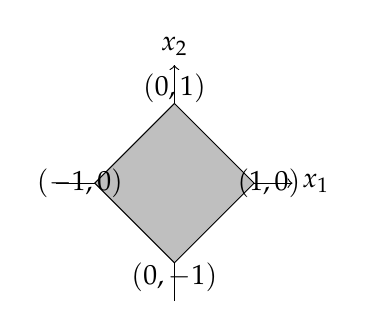
\begin{tikzpicture}
                        \draw[->] (-1.5, 0) -- (1.5, 0) node[right] {$x_1$};
                        \draw[->] (0, -1.5) -- (0, 1.5) node[above] {$x_2$};
                        \draw[thick] (1, 0) -- (0, 1) -- (-1, 0) -- (0, -1) -- cycle;
                        \fill[lightgray] (1, 0) -- (0, 1) -- (-1, 0) -- (0, -1) -- cycle;
                        \node at (1.2, 0) {$(1,0)$};
                        \node at (0, 1.2) {$(0,1)$};
                        \node at (-1.2, 0) {$(-1,0)$};
                        \node at (0, -1.2) {$(0,-1)$};
                    \end{tikzpicture}
                    \caption{Region where $||\mathbf{x}||_1 \leq 1$.}
                    \label{fig:norm1}
                \end{figure}
            \end{soln}
		
		\item 	$||\mathbf{x}||_2 \leq 1$ (Recall that $||\mathbf{x}||_2 =\sqrt{\sum_i x_i^2}$)
			
                \begin{soln}
                    The region corresponding to $||\mathbf{x}||_2 \leq 1$ is a circle centered at the origin with radius 1. This region can be described by the inequality:
                
                    \[
                    \sqrt{x_1^2 + x_2^2} \leq 1,
                    \]
                
                    or equivalently:
                
                    \[
                    x_1^2 + x_2^2 \leq 1.
                    \]
                
                    
                
                    % Example plot using TikZ in LaTeX:
                    \begin{figure}[h!]
                        \centering
                        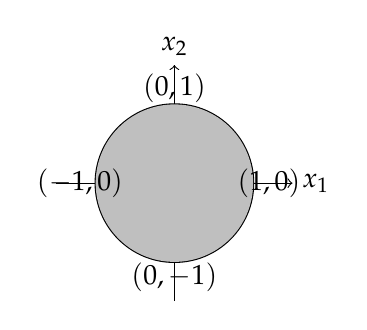
\begin{tikzpicture}
                            \draw[->] (-1.5, 0) -- (1.5, 0) node[right] {$x_1$};
                            \draw[->] (0, -1.5) -- (0, 1.5) node[above] {$x_2$};
                            \draw[thick] (0,0) circle(1);
                            \fill[lightgray] (0,0) circle(1);
                            \node at (1.2, 0) {$(1,0)$};
                            \node at (0, 1.2) {$(0,1)$};
                            \node at (-1.2, 0) {$(-1,0)$};
                            \node at (0, -1.2) {$(0,-1)$};
                        \end{tikzpicture}
                        \caption{Region where $||\mathbf{x}||_2 \leq 1$.}
                        \label{fig:norm2}
                    \end{figure}
                \end{soln}
		\item 	$||\mathbf{x}||_\infty \leq 1$ (Recall that $||\mathbf{x}||_\infty = \max_i |x_i|$)
			
            \begin{soln}
                    The region corresponding to $||\mathbf{x}||_\infty \leq 1$ is a square centered at the origin with side length 2. This region can be described by the inequalities:
                
                    \[
                    -1 \leq x_1 \leq 1
                    \]
                    \[
                    -1 \leq x_2 \leq 1
                    \]
                
                    
                
                    % Example plot using TikZ in LaTeX:
                    \begin{figure}[h!]
                        \centering
                        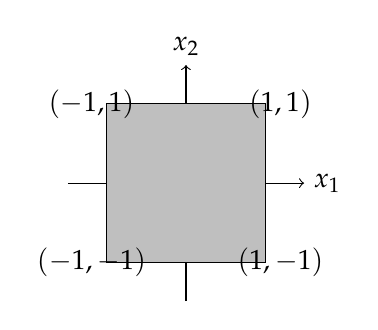
\begin{tikzpicture}
                            \draw[->] (-1.5, 0) -- (1.5, 0) node[right] {$x_1$};
                            \draw[->] (0, -1.5) -- (0, 1.5) node[above] {$x_2$};
                            \draw[thick] (-1, -1) -- (1, -1) -- (1, 1) -- (-1, 1) -- cycle;
                            \fill[lightgray] (-1, -1) -- (1, -1) -- (1, 1) -- (-1, 1) -- cycle;
                            \node at (1.2, 1) {$(1,1)$};
                            \node at (1.2, -1) {$(1,-1)$};
                            \node at (-1.2, -1) {$(-1,-1)$};
                            \node at (-1.2, 1) {$(-1,1)$};
                        \end{tikzpicture}
                        \caption{Region where $||\mathbf{x}||_\infty \leq 1$.}
                        \label{fig:norminfinity}
                    \end{figure}
                \end{soln}
	\end{enumerate}
	
	For $M = \begin{pmatrix}
		5 & 0 & 0 \\ 0 & 7 & 0 \\ 0 & 0 & 3
		
	\end{pmatrix}$, Calculate the following norms.
	\begin{enumerate}\addtocounter{enumi}{3}
		\item $||M||_{2}$ (L2 norm) \\
		
            \begin{soln}
                The $L_2$ norm of a matrix $M$ is given by the largest singular value of $M$. For a diagonal matrix like $M$, the singular values are the absolute values of the diagonal entries. Thus, the $L_2$ norm is the largest diagonal entry.
                \[
                ||M||_{2} = \max \{ |5|, |7|, |3| \} = 7
                \]
            \end{soln}
		
		\item $||M||_{F}$ (Frobenius norm)\\
		  
            \begin{soln}
                The Frobenius norm of a matrix $M$ is computed as the square root of the sum of the absolute squares of its entries. For a diagonal matrix, this is:
                \[
                ||M||_{F} = \sqrt{5^2 + 7^2 + 3^2} = \sqrt{25 + 49 + 9} = \sqrt{83}
                \]
            \end{soln}
		
		
	\end{enumerate}
	
	
	
	\subsection{Geometry [10 pts]}
	Prove the following.  Provide all steps.
	\begin{enumerate}
		\item 	The smallest Euclidean distance from the origin to some point $\mathbf{x}$ in the hyperplane $\mathbf{w}^{T}\mathbf{x} + b = 0$ is $\frac{|b|}{||\mathbf{w}||_2}$.  You may assume $\mathbf{w} \neq 0$.\\
		\begin{soln}

                
                The Euclidean distance from a point $\mathbf{x}$ to the origin is given by $d = \|\mathbf{x}\|_2$. To minimize this distance, we find the perpendicular (shortest) distance between the origin and the hyperplane.
                
                Parametrize the line passing through the origin and orthogonal to the hyperplane
                The normal vector of the hyperplane is $\mathbf{w}$. Any line perpendicular to the hyperplane must be parallel to $\mathbf{w}$. Therefore, we can parametrize any point on this line as:
                \[
                \mathbf{x}(t) = t \mathbf{w}
                \]
                where $t$ is a scalar.

                Substitute $\mathbf{x}(t) = t \mathbf{w}$ into the equation of the hyperplane $\mathbf{w}^T \mathbf{x} + b = 0$:
                \[
                \mathbf{w}^T (t \mathbf{w}) + b = 0
                \]
                \[
                t \mathbf{w}^T \mathbf{w} + b = 0
                \]
                \[
                t \|\mathbf{w}\|_2^2 = -b
                \]
                \[
                t = \frac{-b}{\|\mathbf{w}\|_2^2}
                \]

                Substitute $t = \frac{-b}{\|\mathbf{w}\|_2^2}$ back into the parametrized equation $\mathbf{x}(t) = t \mathbf{w}$:
                \[
                \mathbf{x} = \frac{-b}{\|\mathbf{w}\|_2^2} \mathbf{w}
                \]
                
                \[
                d = \|\mathbf{x}\|_2 = \left\| \frac{-b}{\|\mathbf{w}\|_2^2} \mathbf{w} \right\|_2
                \]
                \[
                d = \frac{|b|}{\|\mathbf{w}\|_2}
                \]
                
                
                \end{soln}
                % \begin{soln}
                    
                    
                %     \begin{enumerate}
                %         \item **Distance Formula**:
                %             The distance from the origin $\mathbf{0}$ to the hyperplane $\mathbf{w}^T \mathbf{x} + b = 0$ is given by:
                %             \[
                %             \text{Distance} = \frac{|\mathbf{w}^T \mathbf{x}_0 + b|}{\|\mathbf{w}\|_2}
                %             \]
                %             For the origin $\mathbf{x}_0 = \mathbf{0}$, this simplifies to:
                %             \[
                %             \text{Distance} = \frac{|b|}{\|\mathbf{w}\|_2}
                %             \]
            
                %         \item **Perpendicular Vector**:
                %             To verify that this is indeed the smallest distance, consider a vector $\mathbf{x}$ that lies on the hyperplane and is perpendicular to $\mathbf{w}$. Choose:
                %             \[
                %             \mathbf{x} = \frac{-b}{\|\mathbf{w}\|_2^2} \mathbf{w}
                %             \]
                %             This vector satisfies:
                %             \[
                %             \mathbf{w}^T \mathbf{x} + b = \mathbf{w}^T \left(\frac{-b}{\|\mathbf{w}\|_2^2} \mathbf{w}\right) + b = \frac{-b \mathbf{w}^T \mathbf{w}}{\|\mathbf{w}\|_2^2} + b = \frac{-b \|\mathbf{w}\|_2^2}{\|\mathbf{w}\|_2^2} + b = 0
                %             \]
                %             Hence, $\mathbf{x}$ lies on the hyperplane.
            
                %         \item **Distance Calculation**:
                %             Calculate the Euclidean norm of $\mathbf{x}$:
                %             \[
                %             \|\mathbf{x}\|_2 = \left\| \frac{-b}{\|\mathbf{w}\|_2^2} \mathbf{w} \right\|_2 = \frac{|b|}{\|\mathbf{w}\|_2^2} \|\mathbf{w}\|_2 = \frac{|b|}{\|\mathbf{w}\|_2}
                %             \]
                %             Thus, the distance from the origin to the hyperplane is:
                %             \[
                %             \frac{|b|}{\|\mathbf{w}\|_2}
                %             \]
                %     \end{enumerate}
                % \end{soln}
		
		\item 	The Euclidean distance between two parallel hyperplane $\mathbf{w}^{T}\mathbf{x} + b_1 = 0$ and $\mathbf{w}^{T}\mathbf{x} + b_2 = 0$ is $\frac{|b_1 - b_2|}{||\mathbf{w}||_2}$ (Hint: you can use the result from the last question to help you prove this one).

            \begin{soln}
            From the previous problem, we know that the shortest distance from the origin to the hyperplane $\mathbf{w}^{T} \mathbf{x} + b = 0$ is given by 
            \[
            d = \frac{|b|}{\|\mathbf{w}\|_2}
            \]
            
            
            Let $\mathbf{x}_1$ and $\mathbf{x}_2$ be points on the two hyperplanes, respectively. Since the hyperplanes are parallel, the normal vector $\mathbf{w}$ is the same for both hyperplanes. The Euclidean distance between the two hyperplanes is simply the difference in their distances from the origin.
            
            Using the result from the previous problem, the distance from the origin to the hyperplane $\mathbf{w}^{T} \mathbf{x} + b_1 = 0$ is:
            \[
            d_1 = \frac{|b_1|}{\|\mathbf{w}\|_2}
            \]
            Similarly, the distance from the origin to the hyperplane $\mathbf{w}^{T} \mathbf{x} + b_2 = 0$ is:
            \[
            d_2 = \frac{|b_2|}{\|\mathbf{w}\|_2}
            \]
            
            \[
            d = \left| \frac{|b_1|}{\|\mathbf{w}\|_2} - \frac{|b_2|}{\|\mathbf{w}\|_2} \right|
            \]
            \[
            d = \frac{|b_1 - b_2|}{\|\mathbf{w}\|_2}
            \]
            
            Thus, the Euclidean distance between the two parallel hyperplanes $\mathbf{w}^T \mathbf{x} + b_1 = 0$ and $\mathbf{w}^T \mathbf{x} + b_2 = 0$ is:
            \[
            d = \frac{|b_1 - b_2|}{\|\mathbf{w}\|_2}
            \]
            
            This distance is minimized because we are measuring along the normal direction, which gives the shortest possible distance between the hyperplanes.
            \end{soln}
  
		 % \begin{soln}
               
   %          The hyperplanes $\mathbf{w}^T \mathbf{x} + b_1 = 0$ and $\mathbf{w}^T \mathbf{x} + b_2 = 0$ are parallel because they have the same normal vector $\mathbf{w}$.
        

   %          Consider a point $\mathbf{x}_1$ on the hyperplane $\mathbf{w}^T \mathbf{x} + b_1 = 0$. The perpendicular distance from the origin to this hyperplane is:
   %              \[
   %              \text{Distance}_{\text{origin to } \mathbf{w}^T \mathbf{x} + b_1 = 0} = \frac{|b_1|}{\|\mathbf{w}\|_2}
   %              \]

   %          The distance from a point on the first hyperplane to the second hyperplane is given by:
   %          \[
   %          \text{Distance} = \frac{|\mathbf{w}^T \mathbf{x} + b_2|}{\|\mathbf{w}\|_2}
   %          \]
   %          Since $\mathbf{x}$ satisfies $\mathbf{w}^T \mathbf{x} + b_1 = 0$, we have $\mathbf{w}^T \mathbf{x} = -b_1$. Therefore:
   %          \[
   %          \text{Distance} = \frac{|-b_1 + b_2|}{\|\mathbf{w}\|_2} = \frac{|b_2 - b_1|}{\|\mathbf{w}\|_2}
   %          \]
   %          Hence, the Euclidean distance between the two parallel hyperplanes $\mathbf{w}^T \mathbf{x} + b_1 = 0$ and $\mathbf{w}^T \mathbf{x} + b_2 = 0$ is:
   %              \[
   %              \frac{|b_1 - b_2|}{\|\mathbf{w}\|_2}
   %              \]

   %          \end{soln}
		
	\end{enumerate}
	
	
\pagebreak
	\section{Programming Skills [10 pts]}
	Sampling from a distribution.  For ea          ch question, submit a scatter plot (you will have 2 plots in total).  Make sure the axes for all plots have the same ranges.
	\begin{enumerate}
		\item Make a scatter plot by drawing 100 items from a two dimensional Gaussian $N((1, -1)^{T}, 2I)$, where I is an identity matrix in $\mathbb{R}^{2 \times 2}$.
		
			\begin{soln}
			% add figure filename, and remove % 
			%    (this can be done by highlighting text and pressing "cmd + /" for sharelatex+mac)
			\begin{figure}[H]
                    \centering
                    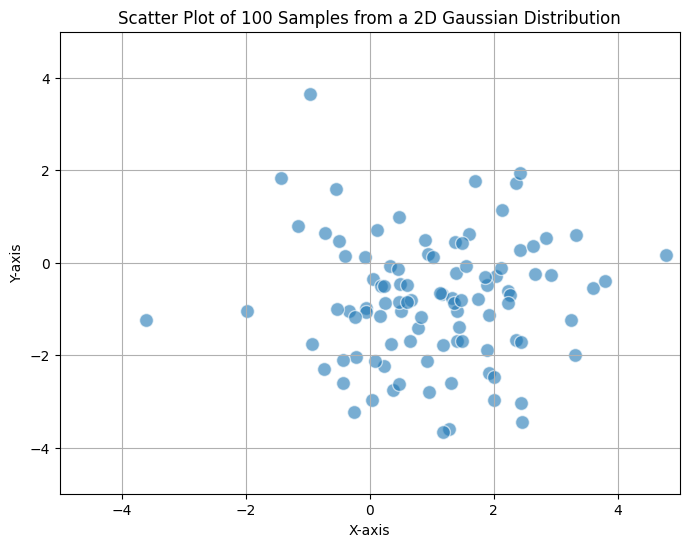
\includegraphics[width=0.6\textwidth]{programming-1.png} % Replace with the actual filename
                    \caption{Scatter Plot of 100 Samples from a Gaussian Distribution}
                    \label{fig:scatter_plot}
                \end{figure}
		\end{soln}
	
		\item Make a scatter plot by drawing 100 items from a mixture distribution 
		$0.3 N\left((5, 0)^{T}, \begin{pmatrix} 1 & 0.25 \\ 0.25 & 1\\ \end{pmatrix}\right)
		+0.7 N\left((-5, 0)^{T}, \begin{pmatrix} 1 & -0.25 \\ -0.25 & 1\\ \end{pmatrix}\right)
		$.
		
		\begin{soln}
		

            \begin{figure}[H]
                \centering
                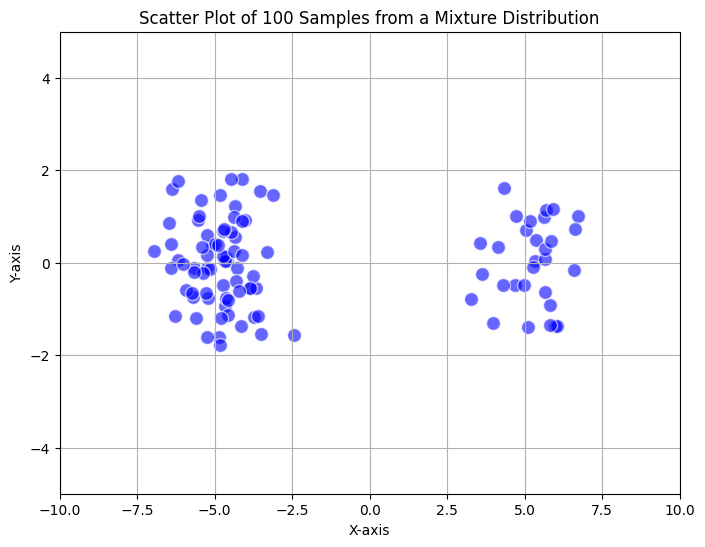
\includegraphics[width=0.6\textwidth]{probability-2.png} % Replace with the actual filename
                \caption{Scatter Plot of 100 Samples from a Mixture                              Distribution}
                \label{fig:scatter_plot}
            \end{figure}
		% add figure filename, and remove % 
		%    (this can be done by highlighting text and pressing "cmd + /" for sharelatex+mac)
		% \begin{figure}[h!]
		%     \centering
		%     \includegraphics[width=0.4\textwidth]{FIGURE_FILENAME.pdf}  
		%             % reference folder/figure.pdf here and adjust width
		%     \captionsetup{labelformat=empty}
		%     \caption{}
		%     \label{fig:my_label}
		% \end{figure}
	\end{soln}
	\end{enumerate}
	
	
	\bibliographystyle{apalike}
	
	
	%----------------------------------------------------------------------------------------
	
	
\end{document}
